% ----------------------------------------------------------------------
%  Pracovní úkoly
% ----------------------------------------------------------------------
\section{Pracovní úkoly}

\textbf{Pracovní úkol 1}

Sestavte malý laboratorní palivový článek pomocí komerčních katalytických GDE (0,3 mgPt cm-2), membrány Nafion NR212 a grafitových bipolárních desek.

\begin{enumerate}
\item Odřízněte dva kusy GDE 2×2 $cm^2$ pomocí nože a pravítka.
\item Odřízněte jeden kus membrány NR-212 7,5×4 $cm^2$.
\item Vytvořte otvory v membráně pro upínací tyče a průchod plynu.
\item Odstraňte z membrány dvě ochranné fólie.
\item Vezměte katodovou bipolární desku.
\item Položte jeden kus GDE na bipolární desku (stranou uhlíkového papíru k průtokovému poli).
\item Zakryjte membránou a zajistěte upevňovacími tyčemi.
\item Umístěte druhý kus GDE (stranou uhlíkového papíru od membrány).
\item Celý systém zakryjte anodovou bipolární deskou.

\end{enumerate}

\textbf{Pracovní úkol 2}

Nastavte experimentální prostředí pro sestavený palivový článek, aktivujte palivový článek (break-in procedure), změřte proudovo-napěťové charakteristiky, prozkoumejte vliv zvlhčování na výkon palivového článku.

\begin{enumerate}
\item Upněte palivový článek pomocí pístu a nastavte upínací tlak 8 barů.
\item Připojte potenciostat pomocí 4-sondového zapojení.
\item Nastavte ohřev palivového článku a zvlhčovacích bubblérů (70 °C).
\item Propláchněte dusíkem obě strany, jak anodu i katodu (5 minut při průtoku N2 100 sccm).
\item Přepněte na H2 na anodové a na O2 na katodové straně (v tomto pořadí); nastavte průtoky 50 sccm; počkejte 10 minut.
\item Nastavte napětí palivového článku; požadované napětí je v rozsahu 0,9-1V.
\item Jakmile je napětí dosaženo a stabilizováno, změřte aktuální napěťovou odezvu palivového článku.
\item Nastavte konstantní napěťovou zátěž 0,4 V po dobu 2 hodin a opakujte měření aktuální napěťové odezvy.
\end{enumerate}

\textbf{Pracovní úkol 3}

Experiment lze provést pomocí edukačního setu FC, který simuluje reálný provoz palivových článků. U tohoto systému je použita architektura s otevřenou katodou. Zaměříme se na teplotu palivového článku. Nastavení teploty lze provést vyvážením zatížení palivového článku a výkonu ventilátoru.

\begin{enumerate}
\item Otevřete vodíkový ventil na tlakové láhvi (ujistěte se, že tlak je snížen na 0,5 baru).
\item Nastavte dobu čištění na 0,5 s a periodu na 60 s.
\item Nastavte výkon ventilátoru na 25\%.
\item Regulujte teplotu FC - nastavením vyšších nebo nižších otáček ventilátoru (PWM Blower \%) se pokuste FC stabilizovat na 40 °C.
\item Zvyšte proud na zátěži o 5 A každých 15 minut a udržujte teplotu svazku FC okolo 40 °C.
\item Při každém proudu sledujte a zaznamenávejte průměrné napětí svazku a výkon ventilátoru.
\item Dosáhněte zatěžovacího proudu 40 A a udržujte jej při stabilní teplotě po dobu 20 minut.
\item Zpomalte ventilátor, abyste dosáhli teploty 50 °C.
\item Změřte průměrné napětí. 
\end{enumerate}

\textbf{Pracovní úkol 4}

Experimenty s palivovým článkem umožňují odhadnout výkon palivového článku, a to jak v případě laboratorního článku, tak setu simulujícího reálný provoz FC. Tyto informace jsou důležité pro odhad výkonu palivových článků a také pro pochopení faktorů, které ovlivňují výkon palivových článků.


\begin{enumerate}
\item Načtěte experimentální data z počítače testovací stanice.
\item Zkopírujte z log souboru data ve sloupcích napětí a proudová hustota.
\item Vyneste graf napětí jako funkce proudu.
\item Najděte hustotu výkonu pro každý proud (součin proudu a napětí) a vykreslete ji.
\item Odhadněte Tafelův sklon pro kinetickou oblast.
\item Vypočítejte ohmické ztráty z lineární části grafu.
\item Odhadněte ztráty při přenosu hmoty jako rozdíl mezi očekávanou lineární závislostí proud-napětí a reálnými datovými body při proudových hustotách > 1,5 A $cm^{-2}$.
\end{enumerate}


% ----------------------------------------------------------------------
%  Teoretická část
% ----------------------------------------------------------------------
\section{Teoretická část}

Vodíkový palivový článek (FC, \textit{fuel cell}) je elektrochemické zařízení, které přeměňuje chemickou energii paliva, v našem případě vodíku, přímo na elektrickou energii, teplo a vodu. Základní konstrukční prvky palivového článku tvoří plynové difúzní elektrody (GDE), protonově vodivá membrána (PEM) a bipolární desky. 

Na anodě probíhá katalytická oxidace vodíku (reakce HOR), při níž se molekula $\mathrm{H_2}$ štěpí na protony a elektrony. Elektrony jsou vedeny vnějším obvodem ke katodě, zatímco protony procházejí protonově vodivou membránou, kde reagují s kyslíkem (reakce ORR) za vzniku vody:

\begin{align}
\text{Anoda:} & \quad \mathrm{2H_2 \rightarrow 4H^+ + 4e^-} \\
\text{Katoda:} & \quad \mathrm{O_2 + 4H^+ + 4e^- \rightarrow 2H_2O}
\end{align}

Tímto procesem vzniká elektrické napětí, jehož hodnota závisí na teplotě, tlaku, koncentraci plynů a vnitřních ztrátách článku. Účinnost systému může při vhodném řízení teploty a zvlhčení dosahovat až 90~\%.

Pro správnou funkci je klíčové zvlhčování membrány, protože protonová vodivost polymeru silně závisí na obsahu vody. Plynové difúzní elektrody zajišťují transport plynů a odvod vznikající vody, zatímco bipolární desky z grafitu nebo kovu zajišťují elektrický kontakt, distribuci plynů a odvod tepla.

Charakteristiku článku lze popsat polarizační křivkou, která vyjadřuje závislost napětí na proudu. Rozlišujeme tři oblasti:

\begin{itemize}
    \item \textbf{Aktivační oblast} -- dominuje přepětí dané kinetikou elektrodových reakcí. Je popsána Tafelovou rovnicí:
    \begin{equation}
    \eta = b \log i,
    \end{equation}
    kde $b$ je Tafelův sklon charakterizující aktivitu katalyzátoru.

    \item \textbf{Ohmická oblast} -- lineární pokles napětí odpovídá vnitřnímu odporu článku. Sklon lineární části polarizační křivky udává velikost ohmických ztrát.

    \item \textbf{Oblast hmotnostní (transportní) polarizace} -- při vysokých proudech dochází k omezenému přenosu plynů a poklesu napětí v důsledku nedostatečné difúze kyslíku nebo akumulace vody v elektrodách.
\end{itemize}

V reálných aplikacích se často využívá architektura s otevřenou katodou, kdy proudící vzduch zajišťuje současně přívod kyslíku i odvod tepla a vody. Takové systémy jsou konstrukčně jednodušší a vhodné pro přenosné zdroje energie, například pro drony nebo malé generátory, avšak jejich řízení teploty a zvlhčení je obtížnější.

% ----------------------------------------------------------------------
%  Výsledky a zpracování měření
% ----------------------------------------------------------------------
\section{Výsledky a zpracování měření}

\subsection{Sestavení článku a měření}

Na základě pracovního úkolu 1 z \cite{bib:zadani} jsme vyrobili vodíkový palivový článek. Ten jsme umístili pomocí pístu do laboratorního stativu. Podle pracovního úkolu 2 jsme proměřili tento článek.

Podle pracovního úkolu 3 jsme použili edukační set FC, který simuluje reálný provoz. Podle zadání jsme měnili parametry článku a naměřené hodnoty jsme znázornili v tabulce \ref{tab:FC-mereni}. Nejprve jsme čekali, než teplota článku dosáhne 40 °C, při níž má nejvyšší efektivitu. Poté jsme postupně zvyšovali zátěž a pomocí nastavení výkonu chlazení se snažili udržet teplotu kolem 40 °C. Určili jsme maximální zatížení článku a poté snížili chlazení tak, aby teplota stoupla na 50 °C. Mimo zahřívání na začátku a na konci jsme hodnoty odečítali po ustálení parametrů jako průměrné hodnoty.

\begin{table}[h!]
\centering
\caption{Naměřené hodnoty pro různé teploty, chlazení a zátěže}
\label{tab:FC-mereni}
\begin{tabular}{
    S[table-format=2.0] % Teplota
    S[table-format=2.0] % Chlazení
    S[table-format=2.2] % Zátěž
    S[table-format=1.4] % Napětí
    S[table-format=2.0] % Výkon
}
\toprule
\textbf{Teplota (°C)} & \textbf{Chlazení (\%)} & \textbf{Zátěž (A)} & \textbf{Napětí (V)} & \textbf{Výkon (W)} \\
\midrule
37 & 20 & 15.00 & 1.6330 & 25 \\
40 & 20 & 15.00 & 1.5930 & 24 \\
40 & 33 & 20.00 & 1.3570 & 27 \\
40 & 42 & 25.00 & 1.1490 & 29 \\
40 & 59 & 30.00 & 0.9110 & 27 \\
40 & 67 & 30.93 & 0.8820 & 27 \\
43 & 30 & 31.70 & 0.9060 & 29 \\
46 & 30 & 30.63 & 0.9872 & 27 \\
50 & 31 & 24.93 & 0.7100 & 18 \\
\bottomrule
\end{tabular}
\end{table}

Vidíme, že maximální hodnota proudu, kterou je tento článek schopný produkovat, je

\begin{equation}
    I_\textbf{max} = 31,7 \; A
\end{equation}

\subsection{Zpracování výsledků}

Na základě pracovního úkolu 4 jsme exportovali data z testovací stanice našeho vyrobeného článku. V grafu \ref{fig:polar-krivk} je znázorněna polarizační křivka a závislost výkonové hustoty na proudové hustotě. Polarizační křivku (označena šedě) můžeme rozdělit do tří oblasti, jak je znázorněno na obrázku modře.


\begin{figure}[!h]
    \centering
    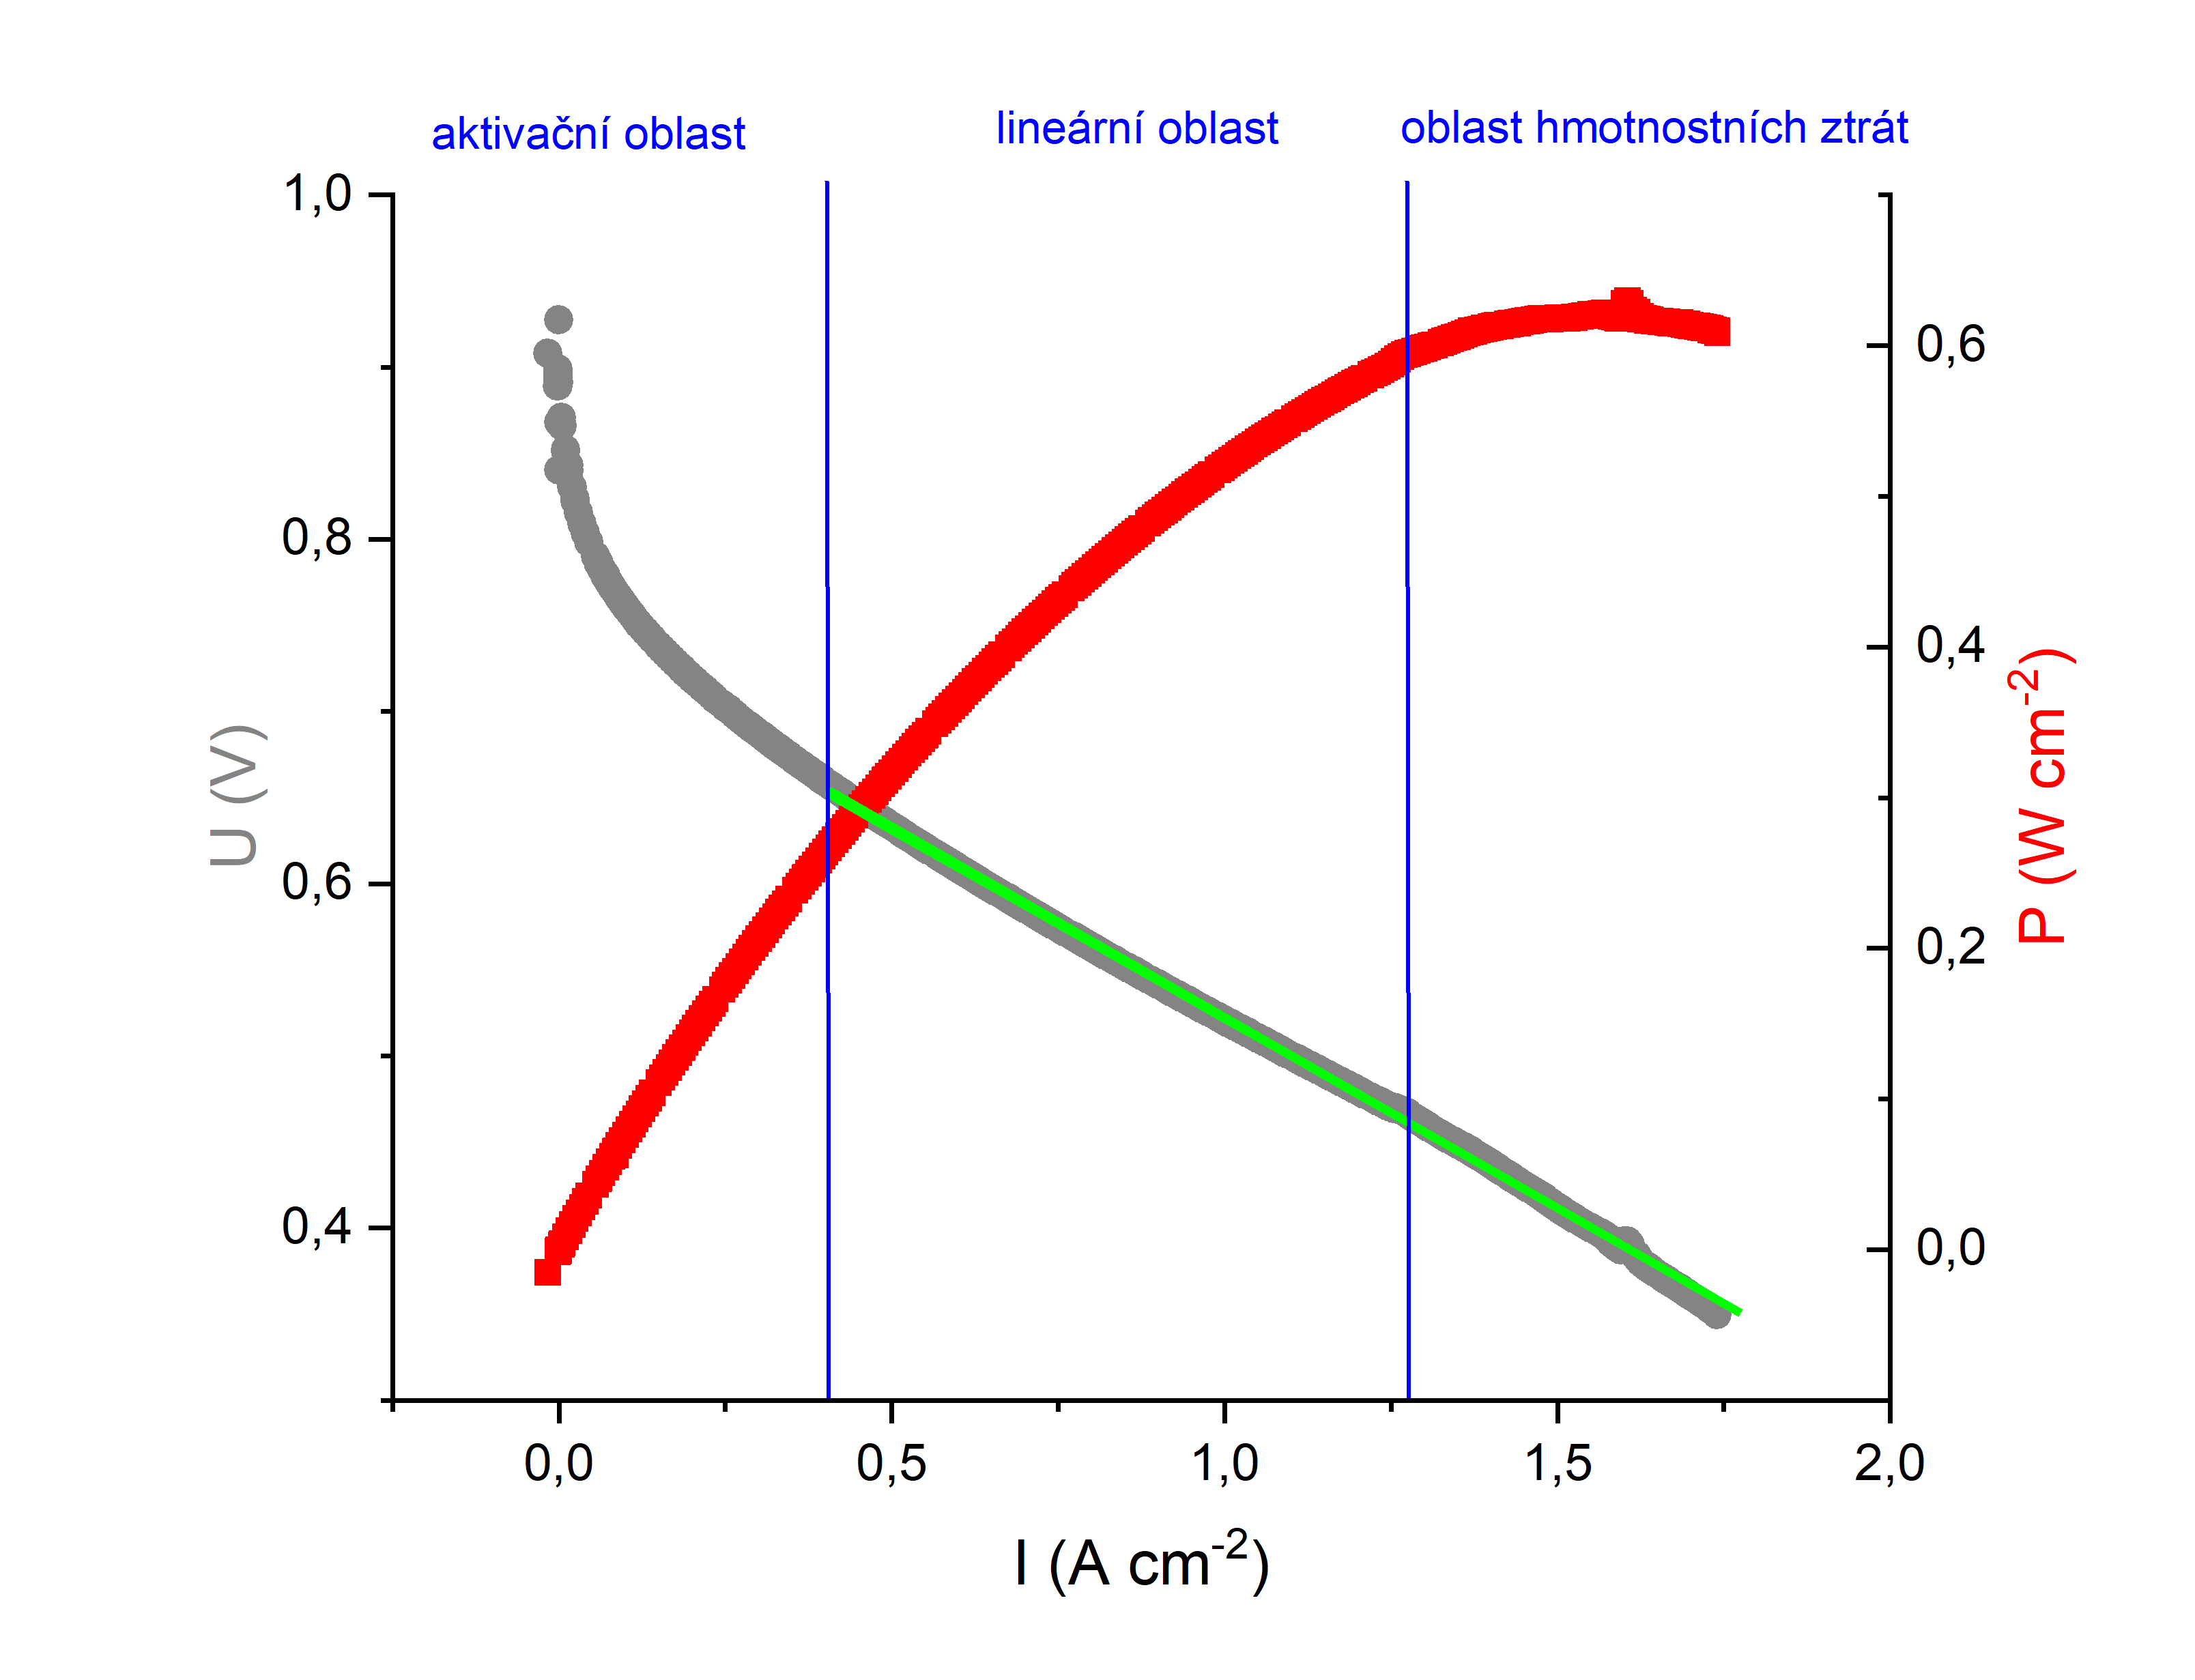
\includegraphics[width=1\linewidth]{H1 - vodíkový palivový článek/Polarizační křivka.png}
    \caption{Polarizační křivka a závislost výkonu}
    \label{fig:polar-krivk}
\end{figure}

Pro kinetickou (aktivační) oblast jsme odhadli Tafelův sklon na základě fitem Tafelovy rovnice (3) podle \cite{bib:studijni-text}. Tento fit je znázorněn v grafu \ref{fig:Tafelův-sklon}. Na osu x jsme vynesli logaritmus z naměřeného proudu a na osu y naměřené přepětí. Tuto závislost jsme fitovali lineární regresí y=ax+b se získanými parametry:

\begin{equation}
    a = -0,1 \; V \; cm^2 \; A^{-1}
\end{equation}

\begin{equation}
    b = 0,6 \; V
\end{equation}

\begin{figure}[!h]
    \centering
    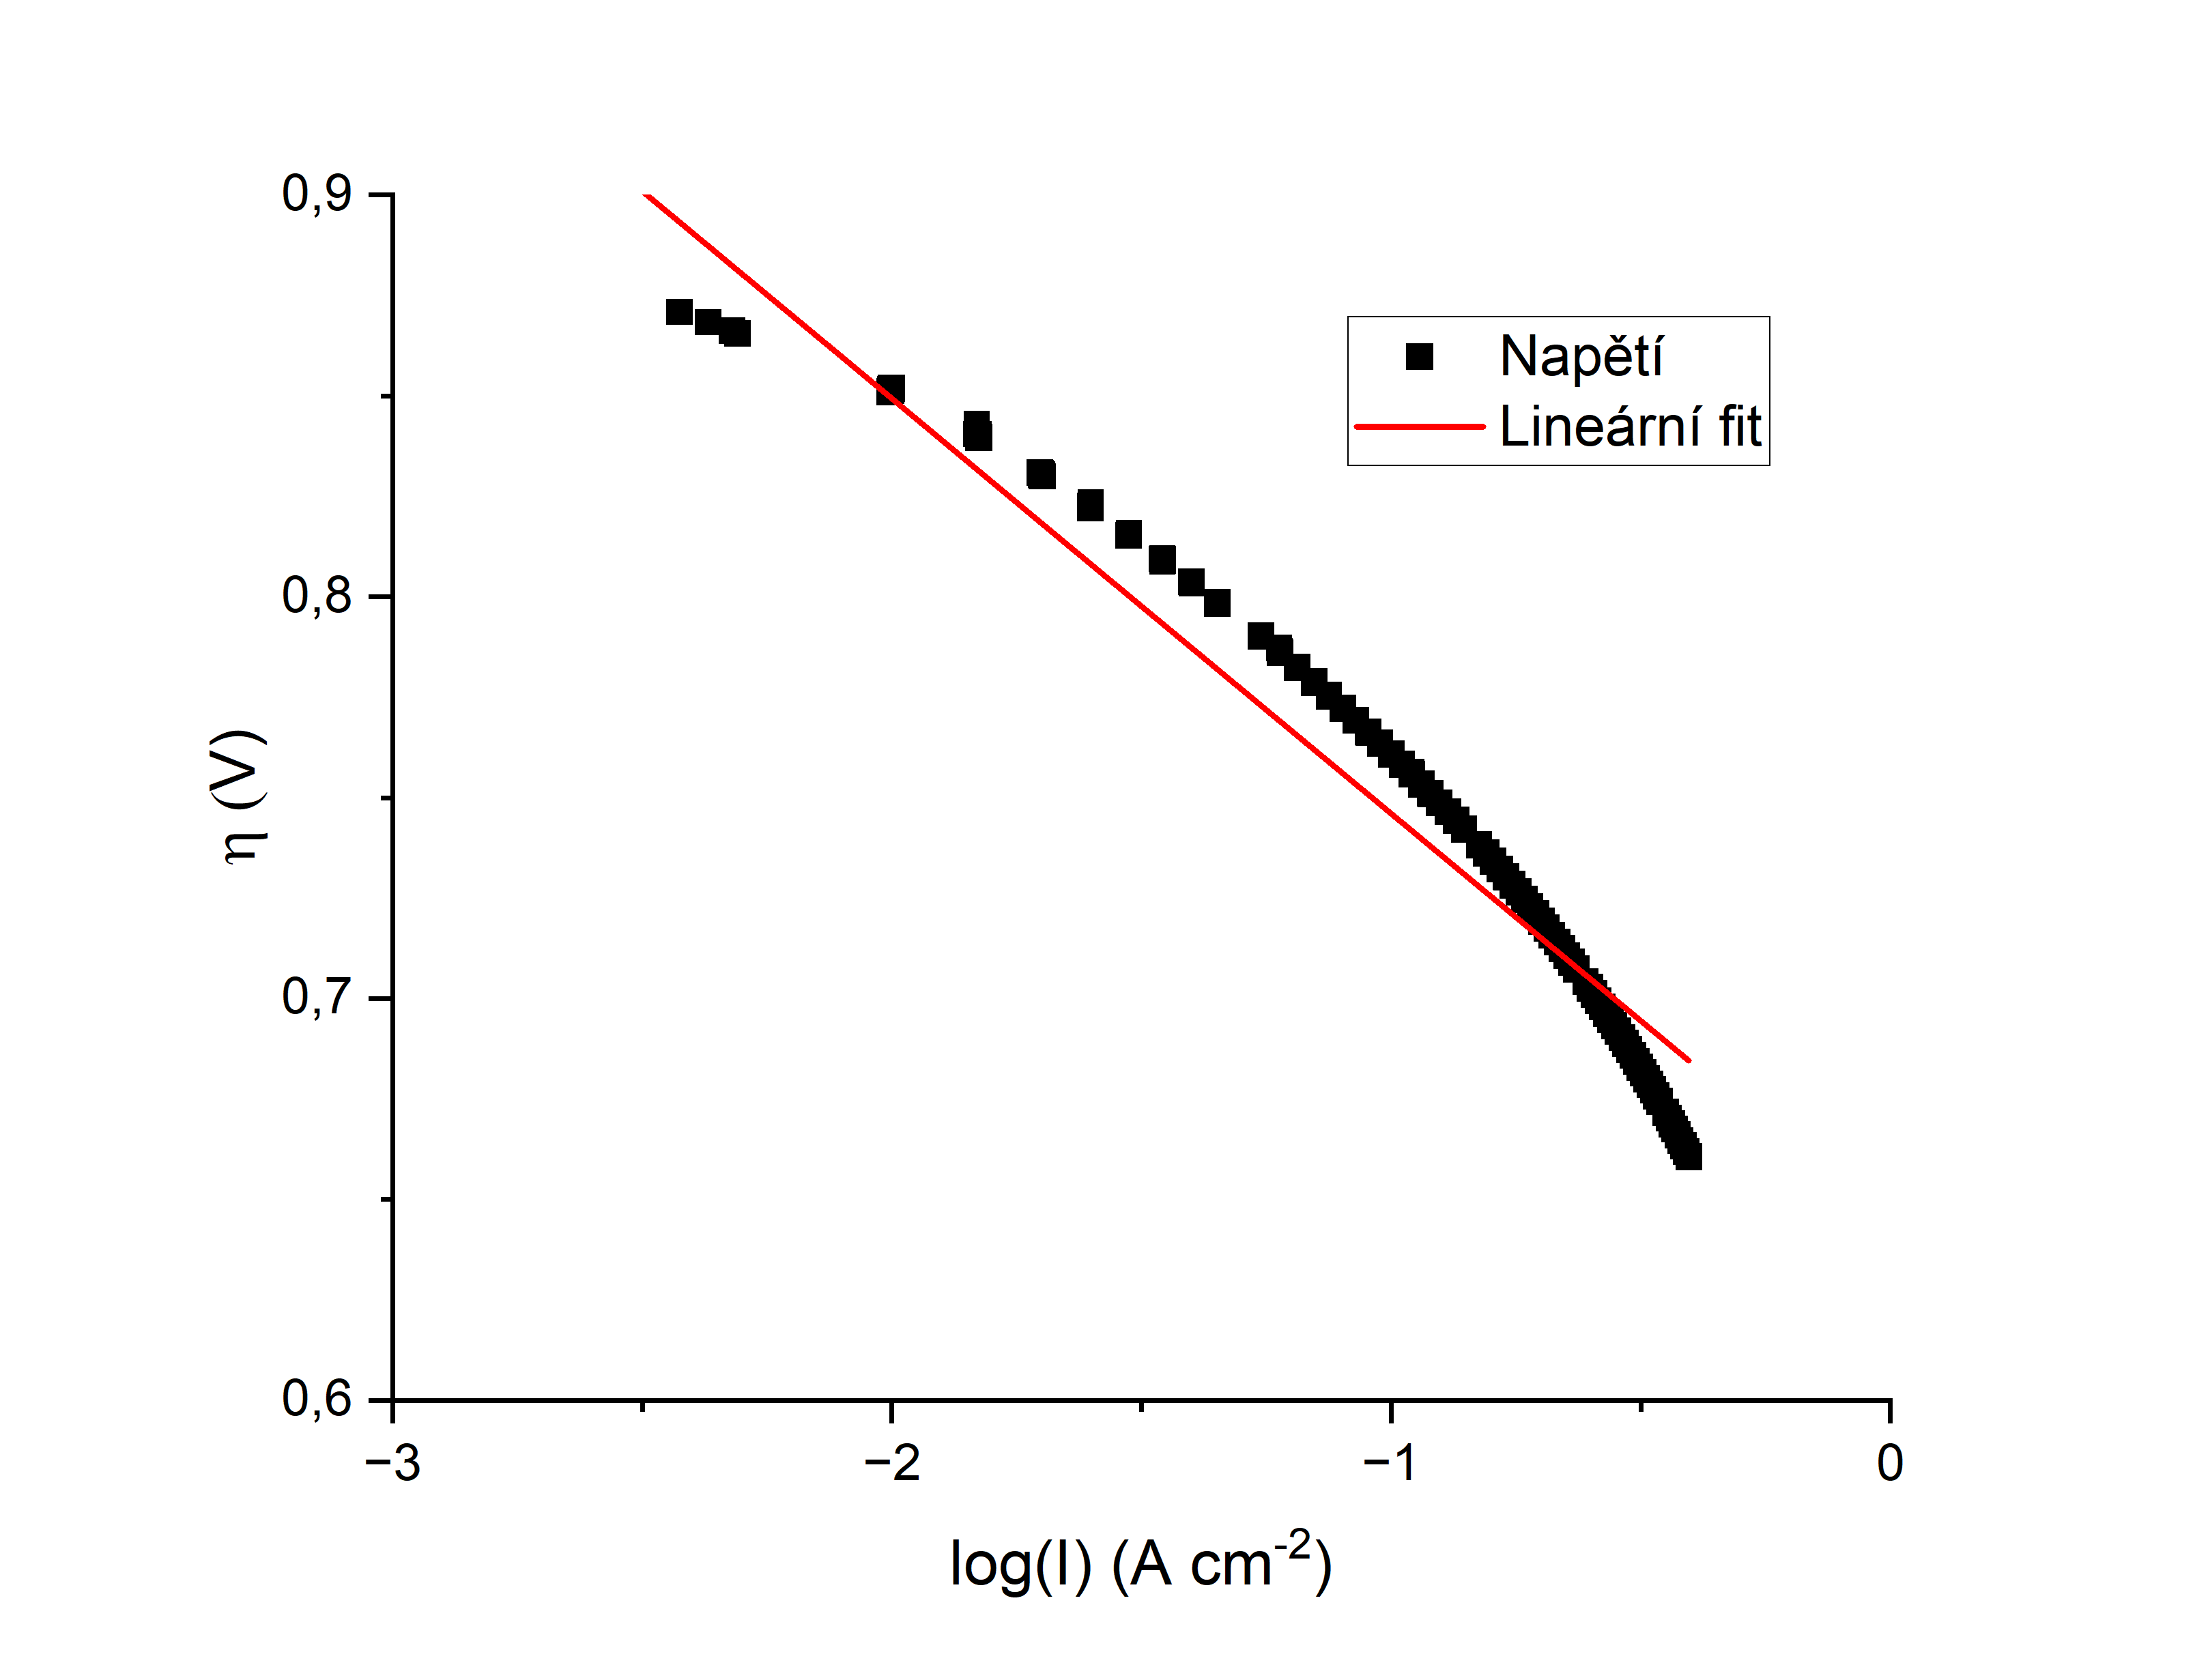
\includegraphics[width=1\linewidth]{H1 - vodíkový palivový článek//Tafelův sklon.png}
    \caption{Tafelův sklon}
    \label{fig:Tafelův-sklon}
\end{figure}

\newpage

Podobně jsme fitovali lineární oblast polarizační křivky lineární funkcí y=ax+b s koeficienty:

 \begin{equation}
     a = -0,2 \; \Omega
 \end{equation}

 \begin{equation}
     b = 0,7 \; V
 \end{equation}

Koeficient a odpovídá ohmickým ztrátám v lineární části grafu.

Nakonec jsme pro oblast hmotnostních ztrát určili pokles napětí, a to 0,02 V oproti očekávané lineární závislosti, která je v grafu znázorněna zeleně. To odpovídá ztrátám při přenosu hmoty.

    
% ----------------------------------------------------------------------
%  Diskuse výsledků
% ----------------------------------------------------------------------			
\newpage
\section{Diskuse výsledků}

Sestavení článku i jeho měření pomocí automatizovaného programu laboratorní stanice proběhlo bez jakýchkoliv komplikací.

Nejistotu měření edukačního článku může způsobit fakt, že naměřené hodnoty jsou průměrné po ustálení stavu článku. Jedná se tedy částečně o odhad ustáleného stavu.

Udávaná maximální zátěžová hodnota edukačního setu je minimálně 40 A, my jsme však změřili maximálně 31, 7 A. To může být způsobeno neznámým stářím setu.

Ověřili jsme, že zvýšením teploty přes optimální mez se výkon článku zhoršuje. To je způsobeno vypařováním se vody z membrány, kterou je třeba stále zvlhčovat pro optimální funkčnost. S rostoucí teplotou rostou ztráty spojené s přenosem hmoty.

Oblast polarizační křivky jsme odhadli podle charakteru křivky v různých bodech. Tento odhad samozřejmě může způsobit změnu fitovaných závislostí a jejich koeficientů. Zejména v oblasti hmotnostních ztrát se tato nepřesnost může projevit. Vizuálně jsou ztráty možná o něco vyšší, než jsme naměřili, avšak takto fitovaná křivka odpovídá lineární oblasti.

% ----------------------------------------------------------------------
%  Závěr
% ----------------------------------------------------------------------
\newpage
\section{Závěr}

V experimentu byl sestaven laboratorní vodíkový palivový článek a proměřeny jeho proudově-napěťové charakteristiky. Na základě získaných dat byla vykreslena polarizační křivka i Tafelův graf (aktivační oblast křivky). Zjištěné hodnoty Tafelova sklonu $a = -0{,}1~\mathrm{V\,cm^2\,A^{-1}}$ a konstanty $b = 0{,}6~\mathrm{V}$ odpovídají předpokládaným hodnotám pro platinový katalyzátor. V lineární oblasti jsme stanovili ohmický odpor $a = -0{,}2~\Omega$ a napěťovou konstantu $b = 0{,}7~\mathrm{V}$. 

Ztráty způsobené omezeným přenosem hmoty se projevily poklesem napětí o přibližně $0{,}02~\mathrm{V}$ oproti ideálnímu lineárnímu průběhu. Maximální proud svazku byl $I_\mathrm{max} = 31{,}7~\mathrm{A}$ při teplotě $40~^\circ\mathrm{C}$, kdy článek dosahoval nejvyšší účinnosti. Při zvýšení teploty na $50~^\circ\mathrm{C}$ došlo k poklesu výkonu v důsledku zhoršeného zvlhčení membrány.

Naměřené výsledky tedy odpovídají teoretickému očekávání: optimální výkon palivového článku je dosažen při správně zvolené teplotě a dostatečné hydrataci membrány, zatímco odchylky vedou ke zvýšení ztrát a poklesu napětí a proudu.
